\section{Zielsetzung}
\label{sec:Ziel}
Es soll der Transport von Wärmeenergie entgegen der Richtung des Wärmeflusses untersucht werden.
Zur Untersuchung der Qualität werden Merkmale wie Güteziffer und Massendurchsatz bestimmt.

\section{Theorie}
\label{sec:Theorie}
Zur Umkehr des Wärmeflusses vom kälteren in ein wärmeres Reservoir benötigt es weitere Energie, zum Beispiel in Form von mechanischer Arbeit.
Diese wird von der Wärmepumpe geleistet.

\subsection{Güteziffer}
\label{sec:Güteziffer}
Das Verhältnis zwischen tranportierter Wärmeenergie $Q_{trans}$ und zu verrichtender Arbeit A:
\begin{equation}
  \nu = \frac{Q_{trans}}{A} \stackrel{\ref{eqn:eqn2}}\Rightarrow \nu_{id} = \frac{T_1}{T_1-T_2}
  \label{eqn:eqn1}
\end{equation}
wird durch die Güteziffer \nu bezeichnet.
Dessen Legitimation ergibt sich aus dem zweiten Hauptsatz der Thermodynamik.
Für realitätsgebundene Berechnungen folgt aus der Irreversibilität der ablaufenden Prozesse, 
dem zweiten Hauptsatz der Thermodynamik und der Annahme, dass sich bei der Wärmeübertragung die Temperaturen der Reservoirs nicht ändern:
\begin{equation}
  \frac{Q_1}{T_1} - \frac{Q_2}{T_2} > 0
  \label{eqn:eqn2}
\end{equation}
Somit ist der Arbeitsaufwand der Pumpe geringer für kleinere Temperaturdifferenzen der beiden Reservoirs.
Die reale Güteziffer \nu lässt sich aus dem Differentialquotienten $\frac{dT_1}{dt}$ für ein Zeitintervall $dt$ bestimmen.
Daraus berechnet sich die Wärmemenge $\frac{dQ_1}{dt}$ zu:
\begin{equation}
  \frac{dQ_1}{dt} = (m_1c_w + m_kc_k) \frac{dT_1}{dt}
  \label{eqn:eqn3}
\end{equation}
Mit $m_1c_w$ für die Wärmekapazität des Wasser in Reservoir 1 und $m_kc_k$ die Wärmekapazität der Kupferschlange und des Eimers.
Somit folgt für die Güteziffer \nu :
\begin{equation}
  \nu = \frac{dQ_1}{dtN} \stackrel{\ref{eqn:eqn2}}\Rightarrow (m_1c_w + m_kc_k) \frac{dT_1}{dt} \cdot \frac{1}{N}
  \label{eqn:eqn4}
\end{equation}
mit N := gemittelte Leistungsaufnahme des Kompressors.

\subsection{Massendurchsatz}
\label{sec:Massendurchsatz}
Der Massendurchsatz berechnet sich nach \cite{AnleitungV206} über den Differentialquotienten über:
\begin{equation}
  \frac{dQ_2}{dt} = (m_2c_w + m_kc_k) \frac{dT_2}{dt}
  \label{eqn:eqn5}
\end{equation}
und
\begin{equation}
  \frac{dQ_2}{dt} = L \frac{dm}{dt}
  \label{eqn:eqn6}
\end{equation}
mit Gl. \ref{eqn:eqn5} und \ref{eqn:eqn6} zu:
\begin{equation}
  (m_2c_w + m_kc_k) \frac{dT_2}{dt} = L \frac{dm}{dt} \Leftrightarrow  \frac{dm}{dt} = (m_2c_w + m_kc_k) \frac{dT_2}{dt \cdot L}
  \label{eqn:eqn7}
\end{equation}
mit bekannter Verdampfungswärme L.

\subsection{Mechanische Kompressorleistung $N_{mech}$}
\label{sec:Kompleistung}
Für die Arbeit $A_m$ gilt bei Verringerung des Gasvolumens von $V_a \textrm{und} V_b$:
\begin{align}
  A_m = - \int_{V_a}^{V_b} pdV
\end{align}
Aus der adiabatischen Kompression des Kompressors, also eine Zustandsänderung ohne Wärmeverluste an die Umgebung, folgt mit der Poissonschen Gleichung und $N_{mech} = \frac{dA_m}{dt}$:
\begin{equation}
  N_{mech} = \frac{1}{\kappa - 1} \left( p_b \sqrt[\kappa]{\frac{p_a}{p_b}} - p_a )\right \frac{dV_a}{dt} = \frac{1}{\kappa - 1} \left( p_b \sqrt[\kappa]{\frac{p_a}{p_b}} - p_a )\right \frac{1}{\rho} \frac{dm}{dt}
  \label{eqn:eqn8}
\end{equation}
mit der Dichte \rho des Gases und dem Druck $p_a$.

\section{Aufbau}
\label{sec:Aufbau}
Eine Wärmepumpe kann schematisch wie folgt dargestellt werden:
\begin{figure}
  \centering
  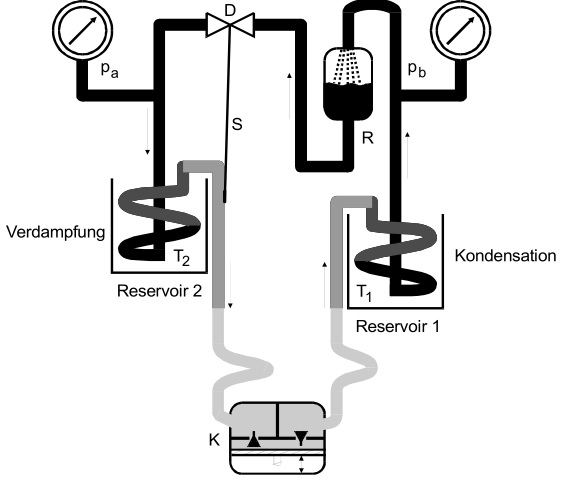
\includegraphics{data/Abb1.jpg}
  \caption{Prinzipieller Aufbau einer Wärmepumpe. \cite{AnleitungV206}}
  \label{fig:Abb1}
\end{figure}
Für die Wärmepumpe wird ein reales Gas benutzt, welches in der Lage ist Wärme während des Verdampfens aufzunehmen und bei der Kondensation abzugeben.
Dies ist die Phasenumwandlungsenergie einer transportablen Energie des Gases.
Für eine ideal arbeitende Pumpe sollte das Gas eine möglichst hohe Kondensationswärme besitzen.
Der Kompressor K sorgt für eine adiabatische Kompression und einen Kreislauf.
Das Druckventil D lässt drickreguliert das Gas durchströmen.
Dort findet sich ein Druckgradient durch die Druckunterschiede in den Reservoiren vor.
Das Gas mit dem Druck $p_b$ und der Temperatur $T_1$ ist flüssig, 
während es auf der anderen Seite bei $p_a$ mit der Temperatur $T_2$ gasförmig ist. 
Wenn sich das Drosselventil D öffnet, entzieht es dem Wasser in Reservoir 2 die Verdampfungswärme L.
Somit folgt, dass das Reservoir 2, das kältere, wärmespendende Gefäß ist.
Das Gas strömt durch den Kompressor K, wird komprimiert und erwärmt sich somit.
Dadurch steigt der Druck im Reservoir $p_a$ , bis sich das Gas verflüssigt und somit Wärme an das Gefäß abgibt.
Mittels weiterer Apparaturen, wie dem Reiniger R werden Blasen durch die Entfernung von Gasresten entfernt,
oder der Steuervorrichtung S, welche das Drossenventil D reguliert. 
Dadurch wird sichergestellt, dass nur Gase in den Kompressor gelangen.